\documentclass[12pt]{article}
\usepackage[margin=0.8in]{geometry}
\usepackage[utf8]{inputenc}
\usepackage{graphicx}
\usepackage[export]{adjustbox}
\usepackage{amsmath}
\usepackage{amsfonts}
\usepackage{amssymb}
\usepackage[version=4]{mhchem}
\usepackage{stmaryrd}
\usepackage{bbold}
%\usepackage[fallback]{xeCJK}
\usepackage{polyglossia}
\usepackage{fontspec}
\usepackage{censor}
%\setCJKmainfont{Noto Serif CJK TC}
\graphicspath{ {../Images/} }
\usepackage{enumitem}
\usepackage{tikz}
\usepackage{pgfplots}
\pgfplotsset{compat=1.18}
\usepackage{amsthm}
\usepackage{tcolorbox}
\usepackage{array}
\usepackage{tabularray}
\usepackage{makecell}
\usepackage{esvect}
%\usepackage{changepage}   % for the adjustwidth environment
\usepackage{enumitem}
\usepackage{tasks}
\usepackage{xcolor}
\usepackage{colortbl}

\tcbuselibrary{theorems}

\definecolor{GrayCen}{HTML}{d2d2d2}
\definecolor{GrayBG}{HTML}{d9d9d9}
\definecolor{BlueDef}{HTML}{104e8b}
\definecolor{GreenProp}{HTML}{025540}
\definecolor{RedMet}{HTML}{cd5556}
\definecolor{BlackSav}{HTML}{000000}
\def\censorcolor{GrayCen}
\let\svcensorrule\censorrule
\renewcommand\censorrule[1]{%
\textcolor{\censorcolor}{\svcensorrule{#1}}}

\newtcbtheorem
[]% init options
{definition}% name
{Définition}% title
{%
  colback=GrayBG,
  colframe=BlueDef,
  fonttitle=\bfseries,
}% options
{def}% prefix

\newtcbtheorem
[]% init options
{proposition}% name
{Proposition}% title
{%
  colback=GrayBG,
  colframe=GreenProp,
  fonttitle=\bfseries,
}% options
{prop}% prefix

\newtcbtheorem
[]% init options
{method}% name
{Méthode}% title
{%
  theorem name,
  colback=GrayBG,
  colframe=RedMet,
  fonttitle=\bfseries,
}% options
{met}% prefix

\newtcbtheorem
[]% init options
{savoir}% name
{Savoir-faire du chapitre}% title
{%
  theorem name,
  colback=GrayBG,
  colframe=BlackSav,
  fonttitle=\bfseries,
}% options
{sav}% prefix

\newtheoremstyle{break}
{\topsep}{\topsep}%
{}{}%
{\bfseries}{}%
{\newline}{}%
\theoremstyle{break}
\newtheorem*{example}{Exemple.}
\newtheorem*{remark}{Remarque.}
\newtheorem*{remarks}{Remarques.}
\newtheorem{rappel}{Rappel}


\newenvironment{demo}[1][\proofname]{%
  \begin{proof}[#1]$ $\newline
  }{%
  \end{proof}
}

\setmainlanguage{french}
%\setmainfont{CMU Serif}

\title{
  \vspace{4em}
  \centering
  \tcbset{colframe=BlackSav,colback=GrayBG}
  \tcbox[tikznode]{
    Chapitre 2 \\Probabilités conditionnelles
  }
}

\author{}
\date{}

\setlength\parindent{0pt}
%\setlist[itemize]{topsep=0pt}
\setlist{nolistsep}
%\setlist[itemize]{noitemsep}
%\setlist[enumerate]{noitemsep}

\newcolumntype{C}[1]{>{\centering\arraybackslash}m{#1}}
\newcolumntype{L}[1]{>{\raggedright\arraybackslash}m{#1}}
\newcolumntype{N}{@{}m{0pt}@{}}

\begin{document}
\maketitle

\tableofcontents

\newsavebox{\hidebox}

% -----------
% Définition de l'environnement qui rend le contenu invisible
\newcommand{\hideM}[1]{\mbox{\vphantom{$#1$}\smash{\colorbox{gray!50}{\phantom{$\displaystyle #1$}}}} }
\newcommand{\hideMW}[1]{\mbox{\vphantom{$#1$}\smash{\colorbox{white}{\phantom{$\displaystyle #1$}}}} }
\newcommand{\hide}[1]{\mbox{\vphantom{#1}\smash{\colorbox{gray!50}{\phantom{#1}}}}}
\NewEnviron{multihide}{%
  \colorbox{gray!50}{
    \begin{lrbox}{\hidebox}%
        \begin{minipage}{\linewidth}%
          \BODY
        \end{minipage}%
    \end{lrbox}%
    % On affiche un espace invisible ayant les dimensions exactes de la boîte
    \vrule width 0pt height \ht\hidebox depth \dp\hidebox\hskip\wd\hidebox%
  }
}
\newcommand{\hidetk}[1]{}
% Définition de l'environnement qui rend le contenu invisible
% \newcommand{\hideM}[1]{\mbox{\vphantom{$#1$}\smash{\colorbox{gray!50}{$\displaystyle #1$}}} }
% \newcommand{\hideMW}[1]{\mbox{\vphantom{$#1$}\smash{\colorbox{white}{$\displaystyle #1$}}} }
% \newcommand{\hide}[1]{\mbox{\vphantom{#1}\smash{\colorbox{gray!50}{#1}}}}
% \NewEnviron{multihide}{%
%   \colorbox{gray!50}{
%     \begin{minipage}{\linewidth}%
%       \BODY
%     \end{minipage}%
%   }
% }
% \newcommand{\hidetk}[1]{#1}
% -----------

\newcommand{\wvec}[1]{\overrightarrow{#1}}
\newcommand{\ssi}[0]{\emph{ssi}\ }
\newcommand{\setR}[0]{$\mathbb{R}$}


\renewcommand{\P}{\mathrm{P}}
\newcommand{\A}{\mathrm{A}}
\newcommand{\B}{\mathrm{B}}

\newpage
\section{Tableaux croisés}

% Tableau croisé d'effectifs par un exemple
% Into tableau de frequences
% calcul de freq marginales, et conditionnelles sans donner le vocabulaire.
% calcul 

Lors d'une campagne de prévention, on interroge $200$ personnes~; pour chacune, on relève son sexe et si elle est fumeuse ou non. Les résultats sont résumés dans le tableau suivant, appelé \emph{tableau croisé d'effectifs} : il croise deux caractères observés sur une même population.
 
\begin{center}
\begin{tabular}{|l|c|c|c|}
\hline
 & \textbf{Fume} & \textbf{Ne fume pas} & \textbf{Total} \\
\hline
\textbf{Hommes} & 36 & 54 & 90 \\
\hline
\textbf{Femmes} & 24 & 86 & 110 \\
\hline
\textbf{Total} & 60 & 140 & 200 \\
\hline
\end{tabular}
\end{center}
 
Pour comparer plus facilement des groupes de tailles différentes, on transforme ce tableau d'effectifs en \emph{tableau de fréquences}, en divisant chaque effectif par l'effectif total de la population ($200$) :
 
%\begin{multihide}
\begin{center}
\begin{tabular}{|l|c|c|c|}
\hline
 & \textbf{Fume} & \textbf{Ne fume pas} & \textbf{Total} \\
\hline
\textbf{Hommes} & 0,18 & 0,27 & 0,45 \\
\hline
\textbf{Femmes} & 0,12 & 0,43 & 0,55 \\
\hline
\textbf{Total} & 0,30 & 0,70 & 1 \\
\hline
\end{tabular}
\end{center}
%\end{multihide}

\paragraph{Lecture par ligne ou par colonne.} Les totaux donnent la répartition de chaque caractère pris isolément.

\begin{example}
   $45\%$ des personnes interrogées sont des hommes, et $30\%$ fument, indépendamment de l'autre caractère.
\end{example}
 
\paragraph{Lecture à l'intérieur d'un groupe.} On peut aussi s'intéresser à un sous-groupe précis.
\begin{example}
Par exemple, parmi les $90$ hommes interrogés, combien fument~? Le tableau d'effectifs indique que $36$ hommes fument, donc la proportion d'hommes fumeurs \emph{parmi les hommes} vaut
\[
\frac{36}{90} = 0{,}4 \quad \text{soit } 40\%.
\]
\end{example}

\begin{remarks}
  \begin{itemize}
    \item Ce nombre est très différent de la fréquence des hommes fumeurs \emph{dans l'ensemble de la population}, qui est 
    $$\dfrac{36}{200}=0{,}18\quad \text{soit } 18\%,$$
    dans un cas, on rapporte l'effectif à $200$, dans l'autre on le rapporte à $90$.
    \item On peut faire le même calcul dans l'autre sens : parmi les $60$ fumeurs, quelle proportion sont des hommes~?
    \[
    \frac{36}{60} = 0{,}6 \quad \text{soit } 60\%.
    \]
    On obtient un nombre différent du précédent : « la proportion d'hommes parmi les fumeurs » n'est pas la même chose que « la proportion de fumeurs parmi les hommes ». Cette remarque sera reprise plus loin.
    \item On obtient les mêmes résultats en utilisant le tableau de fréquences.
  \end{itemize}
 
\end{remarks}
 


\newpage

\section{Rappels sur les probabilités}


%\paragraph{Univers.} 

\begin{definition}{Vocabulaire}{}
  Une \emph{expérience aléatoire} est une expérience dont on ne peut pas prévoir le résultat, mais dont on connaît à l'avance l'ensemble des résultats possibles, appelés \emph{issues}. L'ensemble de toutes les issues est appelé \emph{univers} de l'expérience, noté $\Omega$.
\end{definition}
 
\begin{example}
  \begin{itemize}
    \item[]
    \item On lance un dé à six faces : $\Omega = \{1,2,3,4,5,6\}$.
    \item On tire une carte au hasard dans un jeu de $32$ cartes : $\Omega$ est l'ensemble des $32$ cartes.
  \end{itemize}
\end{example}
 
\begin{definition}{Évènement}{}
  Un \emph{événement} est un sous-ensemble de $\Omega$. Les issues le constituant \emph{réalisent} cet évènement.
\end{definition}
\begin{example}
  Par exemple, pour le lancer de dé, l'événement « obtenir un nombre pair » est le sous-ensemble $\{2,4,6\}$ de $\Omega$.
\end{example}
 
\begin{definition}{Probabilité}{}
Définir une probabilité sur $\Omega=\{e_1,\dots,e_n\}$, c'est associer à chaque issue $e_i$ un nombre $p_i\in[0,1]$ tel que
\[
p_1+p_2+\cdots+p_n = 1.
\]
  Pour un événement $A$, on note $P(A)$ la somme des probabilités des issues qui composent $A$.
\end{definition}


\begin{example}(Sans équiprobabilité)
On lance un dé cubique dont les faces ne sont pas numérotées mais colorées : trois faces rouges, deux faces vertes, et une face bleue. On s'intéresse à la couleur obtenue : $\Omega = \{\text{rouge}, \text{vert}, \text{bleu}\}$. Le dé lui-même est équilibré (chacune de ses six faces a la même probabilité $\frac16$ de sortir), mais les couleurs ne sont pas réparties également sur les faces, donc les issues de $\Omega$ n'ont pas toutes la même probabilité :
\[
P(\text{rouge}) = \frac{3}{6} = 0{,}5, \qquad P(\text{vert}) = \frac{2}{6} = \frac13, \qquad P(\text{bleu}) = \frac{1}{6}.
\]
On vérifie que $P(\text{rouge})+P(\text{vert})+P(\text{bleu})=1$, conformément à la définition. Pour l'événement $A$ « obtenir rouge ou bleu » (rouge et bleu sont incompatibles), on somme directement les probabilités des issues concernées :
\[
P(A) = P(\text{rouge})+P(\text{bleu}) = 0{,}5+\frac16 = \frac23.
\]
% Ici, la formule $\frac{\mathrm{Card}(A)}{\mathrm{Card}(\Omega)}$ n'a pas de sens (elle donnerait $\frac{2}{3}$ pour $\mathrm{Card}(A)=2$ et $\mathrm{Card}(\Omega)=3$, ce qui est juste par coïncidence ici, mais donnerait $\frac13$ pour $P(\text{rouge})$ seul, ce qui est faux) : dès que les issues n'ont pas toutes la même probabilité, il faut revenir à la définition générale et sommer les $p_i$ un par un.
\end{example}

 
\begin{definition}{Cardinal d'un ensemble}{}
  Pour un ensemble fini $A$, on note $\mathrm{Card}(A)$ (ou $|A|$) le nombre d'éléments de $A$.
\end{definition}
 
\begin{remark}
  Lorsque toutes les issues ont la même probabilité, on dit qu'il y a \emph{équiprobabilité}~; chaque issue a alors pour probabilité $\dfrac{1}{\mathrm{Card}(\Omega)}$, et pour tout événement $A$ :
  \[
  P(A) = \frac{\mathrm{Card}(A)}{\mathrm{Card}(\Omega)} = \frac{\text{nombre d'issues favorables à } A}{\text{nombre d'issues possibles}}.
  \]
  Un dé non truqué, une pièce équilibrée ou un paquet de carte bien mélangé sont des situations d'équiprobabilité.
\end{remark}
 
\begin{example}
  On lance un dé équilibré. La probabilité d'obtenir un nombre pair est
  \[
  P(\text{« pair »}) = \frac{\mathrm{Card}(\{2,4,6\})}{\mathrm{Card}(\Omega)} = \frac{3}{6} = 0{,}5.
  \]
\end{example}
 
\subsection{Union, intersection, évènement contraire}
 
\begin{definition}{Union, Intersection}{}
Étant donné deux événements $A$ et $B$ de $\Omega$, on définit les évènements suivants :
\begin{itemize}
  \item $A\cap B$ (« $A$ \emph{et} $B$ ») est réalisé lorsque $A$ et $B$ sont réalisés simultanément~;
  \item $A\cup B$ (« $A$ \emph{ou} $B$ ») est réalisé lorsque au moins un des événements est réalisé.
\end{itemize}
\end{definition}
 
\begin{center}
\begin{tikzpicture}[scale=1]
  \draw (-0.3,-2.1) rectangle (6.3,2.3);
  \node at (-0.05,2) {$\Omega$};
  \begin{scope}[opacity=0.55]
    \fill[blue!40] (2,0) circle (1.6);
    \fill[red!40] (4,0) circle (1.6);
  \end{scope}
  \draw (2,0) circle (1.6);
  \draw (4,0) circle (1.6);
  \node at (1.1,0) {$A$};
  \node at (4.9,0) {$B$};
  \node[font=\small] at (3,0) {$A\cap B$};
\end{tikzpicture}
\end{center}

\begin{proposition}{}{}
  Dans le cas général (les deux événements peuvent avoir des issues communes) :
  \[
  P(A\cup B) = P(A) + P(B) - P(A\cap B).
  \]
\end{proposition}

\begin{remark}
Si $A$ et $B$ n'ont aucune issue commune, on dit qu'ils sont \emph{incompatibles} : $A\cap B=\varnothing$ et
\[
P(A\cup B) = P(A)+P(B).
\]
\end{remark}
 
\begin{minipage}{0.6\linewidth}
\begin{definition}{Évènement contraire}{}
  L'événement contraire de $A$, noté $\overline{A}$, est réalisé lorsque $A$ ne l'est pas. On a :
  \[
  P(\overline{A}) = 1 - P(A).
  \]
\end{definition}
\end{minipage}
\hfill
\begin{minipage}{0.37\linewidth}

\begin{center}
\begin{tikzpicture}[scale=1]
  \draw[fill=gray!20] (-0.3,-1.8) rectangle (5,1.8);
  \fill[white] (2,0) circle (1.4);
  \draw (2,0) circle (1.4);
  \node at (-0.05,1.6) {$\Omega$};
  \node at (2,0) {$A$};
  \node[font=\small] at (3.75,1.4) {$\overline{A}$};
\end{tikzpicture}
\end{center}
  
\end{minipage}
 
\begin{example}
On tire une carte dans un jeu de $52$ cartes. Soit $A$ « tirer un as » et $B$ « tirer un c\oe ur ». On a $P(A)=\frac{4}{52}$, $P(B)=\frac{13}{52}$, et $P(A\cap B)=\frac{1}{52}$ (l'as de c\oe ur). Donc
\[
P(A\cup B) = \frac{4}{52}+\frac{13}{52}-\frac{1}{52} = \frac{16}{52} = \frac{4}{13}.
\]
\end{example} 


% Definition univers (omega) issues evenements
% exemples dé, jeu de carte,...
% Def proba fonction tq somme issues 
% Def Cardinal, def proba evt 
% Ex
% Union intersection proba et graphiques en tikz

\section{Probabilités conditionnelles}

\begin{definition}{Probabilité conditionnelle}{}
  On appelle \textbf{probabilité conditionnelle de ${\mathrm B}$ sachant ${\mathrm A}$}, la probabilité qu'un évènement ${\mathrm B}$ se réalise sachant que l'évènement ${\mathrm A}$ est réalisé. On la note ${\mathrm P}_{\mathrm B}({\mathrm A})$.
\end{definition}

\begin{remark}
  Comme pour les probabilités simples, on a $0 \le {\mathrm P}_{\mathrm B}(\mathrm A) \le 1$.
\end{remark}

\begin{example}(\underline{Activité 1})
  Un laboratoire pharmaceutique a réalisé des tests sur 800 patients atteints d'une maladie.
  Certains sont traités avec le médicament A, d'autres avec le médicament B.
  Le tableau présente les résultats de l'étude :

  \begin{center}
    \begin{tabular}{|c|c|c|c|}
    \hline
    & Médicament A & Médicament B & Total \\
    \hline
    Guéri & 383 & 291 & 674 \\
    \hline
    Non guéri & 72 & 54 & 126 \\
    \hline
    Total & 455 & 345 & 800 \\
    \hline
    \end{tabular}
  \end{center}

  La probabilité que le patient ait pris le médicament A \textbf{sachant qu'il est guéri}
  se note $\mathrm{P}_\mathrm{G}(\mathrm{A})$ et est égale à :

  $$
  \mathrm{P}_\mathrm{G}(\mathrm{A}) = \frac{383}{674} \approx 0{,}57 = 57\,\%.
  $$
\end{example}

\begin{remark}
\begin{itemize}
  \item[]
  \item En général, les mots ``parmi'' ou ``sachant que'' dans un énoncé traduisent des probabilités conditionnelles.
  \item Attention ! Les probabilités conditionnelles $\mathrm{P}_{\mathrm{A}}(\mathrm{B})$ et $\mathrm{P}_{\mathrm{B}}(\mathrm{A})$ ne sont en général pas égales, ici on a :
  $$
  \mathrm{P}_\mathrm{A}(\mathrm{G}) = \frac{383}{455} \approx 0{,}84 = 84\,\%.
  $$
\end{itemize}
\end{remark}

\begin{proposition}{(Admise)}{}~\label{prop:formule_cond}
Soient A et B deux événements avec $\mathrm{P}(\mathrm{A}) \neq 0$.
%\begin{itemize}
%  \item
La probabilité de B sachant A est :

$$
\mathrm{P}_{\mathrm{A}}(\mathrm{~B})=\hideM{\frac{\mathrm{P}(\mathrm{~A} \cap \mathrm{~B})}{\mathrm{P}(\mathrm{~A})}}
$$
%  \item La probabilité de $\mathrm{A} \cap \mathrm{B}$ (``à la fois A et B'') est :
%$$
%\mathrm{P}(\mathrm{A} \cap \mathrm{B})=\hideM{\mathrm{P}_{\mathrm{A}}(\mathrm{B}) \times \mathrm{P}(\mathrm{A})}
%$$
%\end{itemize}
\end{proposition}

% \begin{example}
%   Dans le tableau précédent, on lit l'\emph{effectif} des patients guéri qui ont pris le médicament A à l'intersection de la ligne ``Guéri'' et de la colonne ``Médicament A'' : 383 patients.
%   \begin{itemize}
%     \item On trouve, $\mathrm{P}(\mathrm{A} \cap \mathrm{G}) = \dfrac{383}{800} \approx 0,48$ avec 800 le nombre total de patients.
%     \item De manière similaire, on calcule $\mathrm{P}(\mathrm{G}) = \dfrac{674}{800} \approx 0,84$.
%   \end{itemize}
%   Avec la formule, on retrouve :
%   $$
%   \mathrm{P}_{\mathrm{G}}(\mathrm{~A})={\frac{\mathrm{P}(\mathrm{~G} \cap \mathrm{~A})}{\mathrm{P}(\mathrm{~G})}} = \dfrac{\dfrac{383}{800}}{\dfrac{674}{800}} = \dfrac{383}{674} \approx 0{,}57.
%   $$
% \end{example}
% \begin{proposition}{}{}
% Soient A et B deux événements avec $\mathrm{P}(\mathrm{A}) \neq 0$. Alors,
% 
% $$
% \mathrm{P}(\mathrm{A} \cap \mathrm{B})=\hideM{\mathrm{P}_{\mathrm{A}}(\mathrm{B}) \times \mathrm{P}(\mathrm{A})}
% $$
% \end{proposition}
% \begin{demo}
% On sait que $\mathrm{P}_{\mathrm{A}}(\mathrm{B})=\dfrac{\mathrm{P}(\mathrm{A} \cap \mathrm{B})}{\mathrm{P}(\mathrm{A})}$. Il suffit de multiplier chaque terme de cette égalité par $\mathrm{P}(\mathrm{A})$ pour obtenir le résultat souhaité.
% \end{demo}


\newpage
\subsection{Utilisation des tableaux}

Un tableau à double entrée permet souvent de présenter de façon claire une expérience probabiliste et de calculer facilement des probabilités conditionnelles.

\begin{center}
\renewcommand{\arraystretch}{1.5}
\begin{tabular}{|c|c|c|c|}
\cline { 2 - 4 }
\multicolumn{1}{c|}{} & $\mathrm{B}$ & $\overline{\mathrm{B}}$ & Total \\
\hline
$\mathrm{A}$ & $P(\mathrm{A} \cap \mathrm{B})$ & $P(\mathrm{A} \cap \overline{\mathrm{B}})$ & $P(\mathrm{A})$ \\
\hline
$\overline{\mathrm{A}}$ & $P(\overline{\mathrm{A}} \cap \mathrm{B})$ & $P(\overline{\mathrm{A}} \cap \overline{\mathrm{B}})$ & $P(\overline{\mathrm{A}})$ \\
\hline
Total & $P(\mathrm{B})$ & $P(\overline{\mathrm{B}})$ & 1 \\
\hline
\end{tabular}
\end{center}

\begin{remark}
Dans le tableau ci-dessus $\mathrm{P}(\mathrm{A} \cap \mathrm{B})$ se lit à l'intersection des lignes A et B .

% \begin{itemize}
%   \item $\mathrm{P}(\mathrm{A} \cap \mathrm{B})$ se lit à l'intersection des lignes A et B .
%   \item $\mathrm{P}(\mathrm{A})$ se lit sur la dernière colonne et on a :
% \end{itemize}
% 
% $$
% \mathrm{P}(\mathrm{A})=\mathrm{P}(\mathrm{A} \cap \mathrm{B})+\mathrm{P}(\mathrm{A} \cap \overline{\mathrm{B}}) \quad \text { (formule des probabilités totales) }
% $$
\end{remark}

\begin{example}
Dans une entreprise de 450 salariés, il y a 270 hommes et 180 femmes.
Par ailleurs, les salariés se répartissent en deux catégories : les cadres et les ouvriers.
On sait plus précisément qu'il y a 80 cadres et que le nombre de femmes cadres est de 45.
Quel est le pourcentage d'ouvriers parmi les hommes de l'entreprise ?

Solution :

On réalise le tableau suivant donnant la proportion de salariés pour chaque catégorie (hommes/ femmes et cadres/ouvriers).

\begin{center}
\renewcommand{\arraystretch}{2.5}
\begin{tabular}{|c|c|c|c|}
\cline { 2 - 4 }
\multicolumn{1}{c|}{} & cadres & ouvriers & Total \\
\hline
femmes & $\dfrac{45}{450}$ & $\dfrac{135}{450}$ & $\dfrac{180}{450}$ \\
\hline
hommes & $\dfrac{35}{450}$ & $\dfrac{235}{450}$ & $\dfrac{270}{450}$ \\
\hline
Total & $\dfrac{80}{450}$ & $\dfrac{370}{450}$ & 1 \\
\hline
\end{tabular}
\end{center}

On choisit un salarié au hasard et on considère les événements suivants :\\
H : «Le salarié est un homme»;\\
O : «Le salarié est un ouvrier».\\
Avec ces notations, la proportion cherchée est $\mathrm{P}_{\mathrm{H}}(\mathrm{O})$ :

$$
\mathrm{P}_{\mathrm{H}}(\mathrm{O})=\frac{\mathrm{P}(\mathrm{O} \cap H)}{\mathrm{P}(\mathrm{O})}=\dfrac{\frac{235}{450}}{\frac{270}{450}}=\dfrac{235}{270} \simeq 87 \%
$$
\end{example}

% \begin{example}2026-2027/Secondes/Ch 1 - Vecteurs partie 1/Contrôles/Test AP/def.tex
% Soient A et B deux événements tels que $\mathrm{P}(\mathrm{A})=0,5$ et $\mathrm{P}(\mathrm{A} \cap \mathrm{B})=0,2$. Déterminer $\mathrm{P}_{\mathrm{A}}(\mathrm{B})$.
% 
% ~\\Solution :
% 
% $$
% \mathrm{P}_{\mathrm{A}}(\mathrm{~B})=\frac{\mathrm{P}(\mathrm{~A} \cap \mathrm{~B})}{\mathrm{P}(\mathrm{~A})}=\frac{0,2}{0,5}=0,4
% $$
% \end{example}
% \newpage
% 
% \section{Formule des probabilités totales}
% 
% \begin{proposition}{}{}~\label{prop:pre_tot}
% Soient A et B deux événements avec $\mathrm{P}(\mathrm{A}) \neq 0$, on a :
% \begin{enumerate}
%   \item %La probabilité de $\mathrm{A} \cap \mathrm{B}$ (``à la fois A et B'') est :
% $
% \mathrm{P}(\mathrm{A} \cap \mathrm{B})=\hideM{\mathrm{P}(\mathrm{A}) \times \mathrm{P}_{\mathrm{A}}(\mathrm{B})}
% $
%   \item $\mathrm{P}_{\mathrm{A}}(\mathrm{B}) = 1 - \mathrm{P}_{\mathrm{A}}(\overline{\mathrm{B}})$
% \end{enumerate}
% 
% \end{proposition}
% \begin{proof}
%   \begin{enumerate}
%     \item Se déduit directement de la proposition~\ref{prop:formule_cond}.
%     \item Sachant A, on a nécessairement soit B soit $\overline{\mathrm B}$.
%     Donc $\mathrm{P}_{\mathrm{A}}(\mathrm{B}) + \mathrm{P}_{\mathrm{A}}(\overline{\mathrm{B}}) = 1$, d'où le résultat.
%   \end{enumerate}
% \end{proof}
% 
% \begin{rappel}~\label{rappel:union}
%   Pour tous évènements $\A$ et $\B$, on a :
% 
%   \begin{minipage}{0.5\linewidth}
%     $$ \P(\A \cup \B) = \P(\A) + \P(\B) - \P(\A \cap \B)$$
%     
%   \end{minipage}
%   \begin{minipage}{0.5\linewidth}
%     \begin{tikzpicture}
%       % Univers Omega
%       \draw (-3,-2.2) rectangle (3,2.2);
%       \node at (2.6,1.9) {$\Omega$};
% 
%       % Ombrage : A, B, puis intersection plus foncée
%       \begin{scope}
%         \clip (-3,-2.2) rectangle (3,2.2);
%         \fill[gray!25] (-0.9,0) circle (1.6);
%         \fill[gray!25] (0.9,0) circle (1.6);
%         \begin{scope}
%           \clip (-0.9,0) circle (1.6);
%           \fill[gray!55] (0.9,0) circle (1.6);
%         \end{scope}
%       \end{scope}
% 
%       % Contours
%       \draw (-0.9,0) circle (1.6);
%       \draw (0.9,0) circle (1.6);
% 
%       % Labels
%       \node at (-1.8,0.9) {$A$};
%       \node at (1.8,0.9) {$B$};
%       \node at (0,0) {$A\cap B$};
%     \end{tikzpicture}
%   \end{minipage}
% \end{rappel}
% 
% \begin{proposition}{Formule des probabilités totales.}{}
%   Soient A et B deux évènements avec P(A)$\neq 0$, on a :
%   \begin{align*}
%     \mathrm{P}(\mathrm B) &= \mathrm{P}(\mathrm B \cap \mathrm A) + \mathrm{P}(\mathrm B \cap \overline{\mathrm A}) \\
%     &= \P(\A) \times \mathrm{P}_{\mathrm A}(\mathrm B) + \P(\overline{\A}) \times \mathrm{P}_{\overline{\mathrm A}}(\mathrm B) 
%   \end{align*}
% \end{proposition}
% 
% \begin{proof}
%   \begin{align*}
%     \P(\B) &= \P(\B \cap \Omega)&\\
%     &= \P(\B \cap (\A \cup \overline{\A}))&\\
%     %&= \P((\B \cap \A) \cup  (\B \cap \overline{\A}))& (\text{Rappel.~\ref{rappel:union} et } \P(\A \cap \overline{\A}) = 0)\\
%     &= \P(\B \cap \A) + \P(\B \cap \overline{\A})&(\text{Rappel.~\ref{rappel:union} et } \P(\A \cap \overline{\A}) = 0)\\
%     &= \P(\A) \times \P_{\A}(\B)+ \P(\overline{\A}) \times \P_{\overline{\A}}(\B)&
%   \end{align*}
% \end{proof}
% 
% \begin{center}
%   \begin{tikzpicture}[scale=0.8]
%     % Univers Omega (grande ellipse)
%     \draw (0,0) ellipse (4 and 1.8);
%     \node at (3.5,1.4) {$\Omega$};
% 
%     % Frontière ondulée entre A et son complémentaire
%     \draw (0,1.8) .. controls (0.4,1.1) and (-0.4,-1.1) .. (0,-1.8);
% 
%     % Labels des deux parties de la partition
%     \node at (-2,1) {$A$};
%     \node at (2,1) {$\overline{A}$};
% 
%     % Événement B (ellipse grisée traversant la partition)
%     \begin{scope}
%       \clip (0,0) ellipse (4 and 2.2);
%       \fill[gray!40] (0,-0.3) ellipse (3.3 and 0.9);
%     \end{scope}
%     \draw (0,-0.3) ellipse (3.3 and 0.9);
%     \node at (0,-0.3) {$B$};
%   \end{tikzpicture}
% \end{center}
% 
% \begin{example}
% Soient A et B deux événements tels que $\mathrm{P}(\mathrm{A})=0,6, \mathrm{P}_{\mathrm{A}}(\mathrm{B})=0,5$ et $\mathrm{P}_{\overline{\mathrm{A}}}(\mathrm{B})=0,1$.\\
% Déterminer $\mathrm{P}(\mathrm{B})$.
% 
% ~\\Solution :
% 
% On sait que $\mathrm{P}(\overline{\mathrm{A}})=1-\mathrm{P}(\mathrm{A})=0,4$.% Par ailleurs, comme A et $\overline{\mathrm{A}}$ forment une partition de l'univers, on peut appliquer la formule des probabilités totales :
% 
% $$
% \begin{aligned}
% \mathrm{P}(\mathrm{B}) & =\mathrm{P}(\overline{\mathrm{A}} \cap \mathrm{~B})+\mathrm{P}(\mathrm{A} \cap \mathrm{B}) \\
% & =\mathrm{P}(\overline{\mathrm{A}}) \times \mathrm{P}_{\overline{\mathrm{A}}}(\mathrm{B})+\mathrm{P}(\mathrm{A}) \times \mathrm{P}_{\mathrm{A}}(\mathrm{B}) \\
% & =0,4 \times 0,1+0,6 \times 0,5 \\
% & =0,34
% \end{aligned}
% $$
% \end{example}
% 
% % \begin{remark}
% %   En multipliant l'égalité $1 = \mathrm{P}_{\mathrm{A}}(\mathrm{B}) + \mathrm{P}_{\mathrm{A}}(\overline{\mathrm{B}}) = 1$ par P(A), on obtient :
% %   \begin{align*}
% %     \mathrm{P}(\mathrm A) &= \left[ \mathrm{P}_{\mathrm{A}}(\mathrm{B}) + \mathrm{P}_{\mathrm{A}}(\overline{\mathrm{B}}) \right] \times \mathrm{P}(\mathrm A)&\\
% %     &= \mathrm{P}_{\mathrm{A}}(\mathrm{B}) \times \mathrm{P}(\mathrm A) + \mathrm{P}_{\mathrm{A}}(\overline{\mathrm{B}}) \times \mathrm{P}(\mathrm A)&\\
% %     &= \mathrm{P}(\mathrm{A} \cap \mathrm{B}) + \mathrm{P}(\mathrm{A} \cap \overline{\mathrm{B}})& \text{(Prop.~\ref{prop:pre_tot}.1)}
% %   \end{align*}
% % \end{remark}
% % 
% % \begin{definition}{}{}
% % Soit $n \geqslant 2$. Soient $\mathrm{A}_{1}, \mathrm{~A}_{2}, \ldots,, \mathrm{~A}_{n}$ des événements non vides. On dit qu'ils forment une partition de l'univers $\Omega$ lorsque les conditions suivantes sont vérifiées :
% % 
% % \begin{itemize}
% %   \item Ils sont deux à deux incompatibles : pour tous $i \neq j, \hideM{\mathrm{A}_{i} \cap \mathrm{A}_{j}=\emptyset}$;
% %   \item $\mathrm{A}_{1} \cup \mathrm{A}_{2} \cup \ldots \cup \mathrm{A}_{n}=\hideM{\Omega}$
% % \end{itemize}
% % \end{definition}
% % 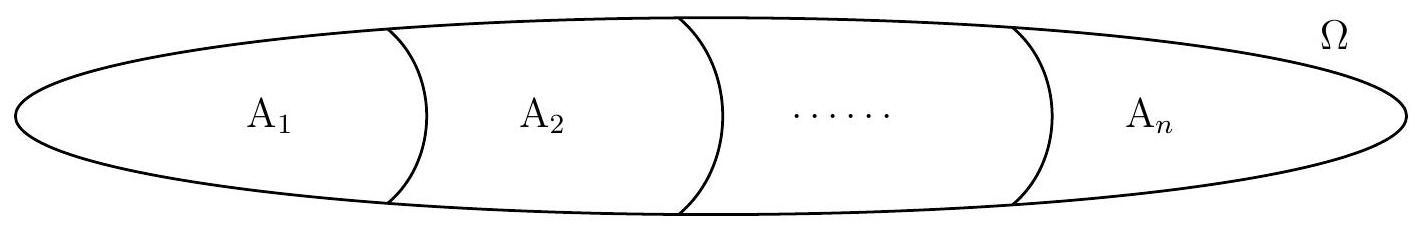
\includegraphics[max width=0.85\textwidth, center]{2025_05_13_795d2fb7a2e4fd469256g-2}
% % 
% % \begin{example}
% % On lance un dé à six faces. L'univers est $\Omega=\{1 ; 2 ; 3 ; 4 ; 5 ; 6\}$.\\
% % On considère les événements suivants :\\
% % A : «Obtenir un résultat pair»;\\
% % B : «Obtenir un 5 »;\\
% % C : «Obtenir un 1 ou un 3 ».\\
% % Les événements $\mathrm{A}, \mathrm{B}$ et $C$ forment ainsi une partition de l'univers.
% % \end{example}
% % 
% % \begin{remark}
% % Si A est un événement de probabilité non nulle, alors A et $\overline{\mathrm{A}}$ forment une partition de l'univers car :
% % 
% % \begin{itemize}
% %   \item $\mathrm{A} \cap \overline{\mathrm{A}}=\emptyset$;
% %   \item $\mathrm{A} \cup \overline{\mathrm{A}}=\Omega$.
% % \end{itemize}
% % \end{remark}
% % 
% % \begin{proposition}{}{Formule des probabilités totales}
% % Soit $n \geqslant 2$. Soient $\mathrm{A}_{1}, \mathrm{A}_{2}, \ldots, \mathrm{A}_{n}$ des événements formant une partition de l'univers et soit B un événement. Alors,
% % 
% % $$
% % \begin{aligned}
% % \mathrm{P}(\mathrm{B}) & =\mathrm{P}\left(\mathrm{A}_{1} \cap \mathrm{B}\right)+\mathrm{P}\left(\mathrm{A}_{2} \cap \mathrm{B}\right)+\ldots+\mathrm{P}\left(\mathrm{A}_{n} \cap \mathrm{B}\right) \\
% % & =\mathrm{P}\left(\mathrm{A}_{1}\right) \times \mathrm{P}_{\mathrm{A}_{1}}(\mathrm{B})+\mathrm{P}\left(\mathrm{A}_{2}\right) \times \mathrm{P}_{\mathrm{A}_{2}}(\mathrm{B})+\ldots+\mathrm{P}\left(\mathrm{A}_{n}\right) \times \mathrm{P}_{\mathrm{A}_{n}}(\mathrm{B})
% % \end{aligned}
% % $$
% % \end{proposition}
% % 
% \begin{remark}
%   La \textbf{formule des probabilités totales} peut être étendue à plusieurs évènements $\A_1, \dots, \A_n$ non vides formant une \textbf{partition de l'univers}. C'est-à-dire, tels que :
%   \begin{enumerate}
%     \item ils sont deux à deux incompatibles : pour tous $i \neq j$, $\A_i \cap \A_j = \emptyset$;
%     \item ils recouvrent tout l'univers : $A_1 \cap A_2 \cap \dots \cap \A_n = \Omega$.
%   \end{enumerate}
% \end{remark}
% \begin{center}
% 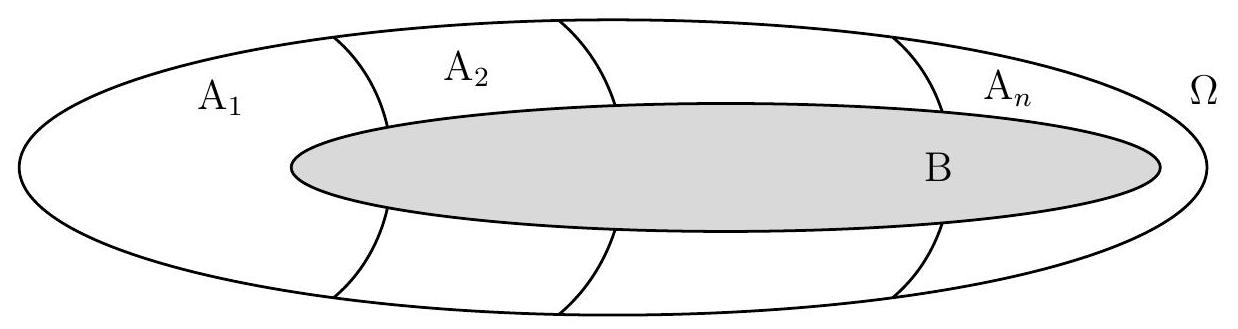
\includegraphics[max width=0.6\textwidth]{2025_05_13_795d2fb7a2e4fd469256g-3}
% 
% On a alors :
% $$
% \begin{aligned}
% \mathrm{P}(\mathrm{B}) & =\mathrm{P}\left(\mathrm{A}_{1} \cap \mathrm{B}\right)+\mathrm{P}\left(\mathrm{A}_{2} \cap \mathrm{B}\right)+\ldots+\mathrm{P}\left(\mathrm{A}_{n} \cap \mathrm{B}\right) \\
% & =\mathrm{P}\left(\mathrm{A}_{1}\right) \times \mathrm{P}_{\mathrm{A}_{1}}(\mathrm{B})+\mathrm{P}\left(\mathrm{A}_{2}\right) \times \mathrm{P}_{\mathrm{A}_{2}}(\mathrm{B})+\ldots+\mathrm{P}\left(\mathrm{A}_{n}\right) \times \mathrm{P}_{\mathrm{A}_{n}}(\mathrm{B})
% \end{aligned}
% $$
% \end{center}
% 
% %\begin{demo}
% %Soit $n \geqslant 2$. Soient $\mathrm{A}_{1}, \mathrm{~A}_{2}, \ldots, \mathrm{~A}_{n}$ des événements formant une partition de l'univers et soit B un événement. Alors,
% %
% %$$
% %\begin{aligned}
% %\mathrm{P}(\mathrm{~B}) & =\mathrm{P}(\mathrm{~B} \cap \Omega) \\
% %& =\mathrm{P}\left(\mathrm{~B} \cap\left(\mathrm{~A}_{1} \cup \mathrm{~A}_{2} \cup \ldots \cup \mathrm{~A}_{n}\right)\right) \\
% %& =\mathrm{P}\left(\left(\mathrm{~B} \cap \mathrm{~A}_{1}\right) \cup\left(\mathrm{B} \cap \mathrm{~A}_{2}\right) \cup \ldots \cup\left(\mathrm{B} \cap \mathrm{~A}_{n}\right)\right) \\
% %& =\mathrm{P}\left(\mathrm{~B} \cap \mathrm{~A}_{1}\right)+\mathrm{P}\left(\mathrm{~B} \cap \mathrm{~A}_{2}\right)+\ldots+\mathrm{P}\left(\mathrm{~B} \cap \mathrm{~A}_{n}\right)
% %\end{aligned}
% %$$
% %
% %car les événements $\mathrm{A}_{i}$ sont deux à deux disjoints donc les événements $\mathrm{A}_{i} \cap \mathrm{~B}$ aussi. Pour montrer la deuxième égalité, on utilise ensuite le fait que, pour tout entier $i$,
% %
% %$$
% %\mathrm{P}\left(\mathrm{~B} \cap \mathrm{~A}_{i}\right)=\mathrm{P}\left(\mathrm{~A}_{i}\right) \times \mathrm{P}_{\mathrm{A}_{i}}(\mathrm{~B})
% %$$
% %
% %Ainsi, on obtient bien :
% %
% %$$
% %\mathrm{P}(\mathrm{~B})=\mathrm{P}\left(\mathrm{~A}_{1}\right) \times \mathrm{P}_{\mathrm{A}_{1}}(\mathrm{~B})+\mathrm{P}\left(\mathrm{~A}_{2}\right) \times \mathrm{P}_{\mathrm{A}_{2}}(\mathrm{~B})+\ldots+\mathrm{P}\left(\mathrm{~A}_{n}\right) \times \mathrm{P}_{\mathrm{A}_{n}}(\mathrm{~B})
% %$$
% %\end{demo}
% 
% 
% %\section{Calcul des probabilités conditionnelles en pratique}
% %\subsection{Utilisation des tableaux}
% %
% %Un tableau à double entrée permet souvent de présenter de façon claire une expérience probabiliste et de calculer facilement des probabilités conditionnelles.
% %
% %\begin{center}
% %\renewcommand{\arraystretch}{1.5}
% %\begin{tabular}{|c|c|c|c|}
% %\cline { 2 - 4 }
% %\multicolumn{1}{c|}{} & $\mathrm{B}$ & $\overline{\mathrm{B}}$ & Total \\
% %\hline
% %$\mathrm{A}$ & $P(\mathrm{A} \cap \mathrm{B})$ & $P(\mathrm{A} \cap \overline{\mathrm{B}})$ & $P(\mathrm{A})$ \\
% %\hline
% %$\overline{\mathrm{A}}$ & $P(\overline{\mathrm{A}} \cap \mathrm{B})$ & $P(\overline{\mathrm{A}} \cap \overline{\mathrm{B}})$ & $P(\overline{\mathrm{A}})$ \\
% %\hline
% %Total & $P(\mathrm{B})$ & $P(\overline{\mathrm{B}})$ & 1 \\
% %\hline
% %\end{tabular}
% %\end{center}
% %
% %\begin{remark}
% %Dans le tableau ci-dessus:
% %
% %\begin{itemize}
% %  \item $\mathrm{P}(\mathrm{A} \cap \mathrm{B})$ se lit à l'intersection des lignes A et B .
% %  \item $\mathrm{P}(\mathrm{A})$ se lit sur la dernière colonne et on a :
% %\end{itemize}
% %
% %$$
% %\mathrm{P}(\mathrm{A})=\mathrm{P}(\mathrm{A} \cap \mathrm{B})+\mathrm{P}(\mathrm{A} \cap \overline{\mathrm{B}}) \quad \text { (formule des probabilités totales) }
% %$$
% %\end{remark}
% %
% %\begin{example}
% %Dans une entreprise de 450 salariés, il y a 270 hommes et 180 femmes. Par ailleurs, les salariés se répartissent en deux catégories : les cadres et les ouvriers. On sait plus précisément qu'il y a 80 cadres et que le nombre de femmes cadres est de 45. Quel est le pourcentage d'ouvriers parmi les hommes de l'entreprise?
% %
% %\newpage
% %Solution :
% %
% %On réalise le taleau suivant donnant la proportion de salariés pour chaque catégorie (hommes/ femmes et cadres/ouvriers).
% %
% %\begin{center}
% %\renewcommand{\arraystretch}{3}
% %\begin{tabular}{|c|c|c|c|}
% %\cline { 2 - 4 }
% %\multicolumn{1}{c|}{} & cadres & ouvriers & Total \\
% %\hline
% %femmes & $\dfrac{45}{450}$ & $\dfrac{135}{450}$ & $\dfrac{180}{450}$ \\
% %\hline
% %hommes & $\dfrac{35}{450}$ & $\dfrac{235}{450}$ & $\dfrac{270}{450}$ \\
% %\hline
% %Total & $\dfrac{80}{450}$ & $\dfrac{370}{450}$ & 1 \\
% %\hline
% %\end{tabular}
% %\end{center}
% %
% %On choisit un salarié au hasard et on considère les événements suivants :\\
% %H : «Le salarié est un homme»;\\
% %O : «Le salarié est un ouvrier».\\
% %Avec ces notations, la proportion cherchée est $\mathrm{P}_{\mathrm{H}}(\mathrm{O})$ :
% %
% %$$
% %\mathrm{P}_{\mathrm{H}}(\mathrm{O})=\frac{\mathrm{P}(\mathrm{O} \cap H)}{\mathrm{P}(\mathrm{O})}=\dfrac{\frac{235}{450}}{\frac{270}{450}}=\dfrac{235}{270} \simeq 87 \%
% %$$
% %\end{example}
% %
% %
% \newpage
% \subsection{Utilisation des arbres}
% Un arbre de probabilité est un autre moyen de représenter efficacement une situation probabiliste et de calculer des probabilités conditionnelles.\\
% 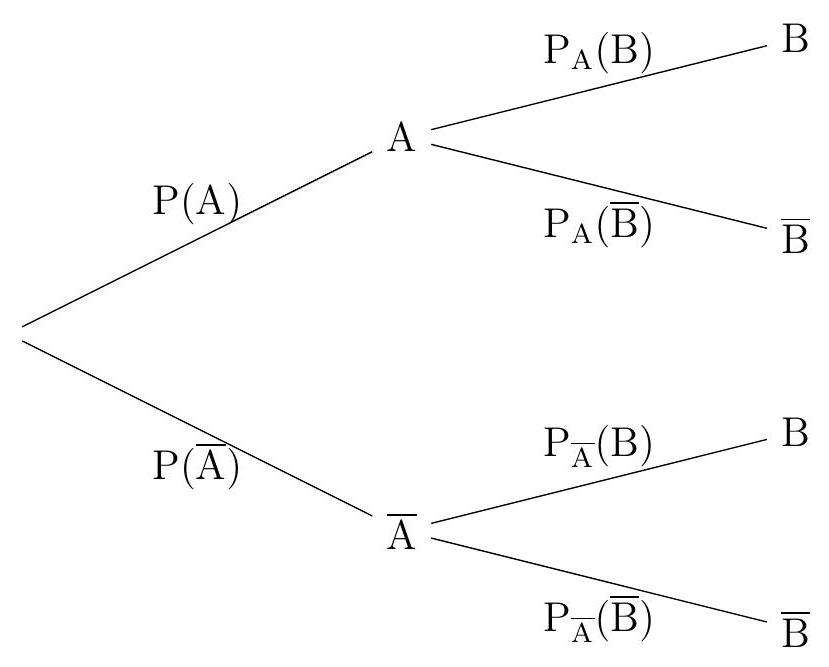
\includegraphics[max width=0.35\textwidth, center]{2025_05_13_795d2fb7a2e4fd469256g-5}
% \vspace{-3em}
% \begin{remark}
% \begin{itemize}
%   \item[]
%   \item La somme des probabilités des chemins issues d'un noeud est égale à 1 .
% 
% Par exemple, $\mathrm{P}(\mathrm{A})+\mathrm{P}(\overline{\mathrm{A}})=1$ et $\mathrm{P}_{\mathrm{A}}(\mathrm{B})+\mathrm{P}_{\mathrm{A}}(\overline{\mathrm{B}})=1$.
% 
%   \item La probabilité d'un chemin est la probabilité de l'intersection des événements que comporte ce chemin. Elle se calcule en multipliant les probabilités du chemin.\\
% Par exemple, $\mathrm{P}(\mathrm{A} \cap \mathrm{B})=\mathrm{P}(\mathrm{A}) \times \mathrm{P}_{\mathrm{A}}(\mathrm{B}) \quad$ (d'après la propriété 1 ).
%   \item La probabilité d'un événement est égale à la somme des chemins conduisant à cet événement.\\
% Par exemple, $\mathrm{P}(\mathrm{B})=\mathrm{P}(\mathrm{A} \cap \mathrm{B})+\mathrm{P}(\overline{\mathrm{A}} \cap \mathrm{B}) \quad$ (d'après la formule des probabilités totales)
% \end{itemize}
% \end{remark}
% 
% \begin{example}
% On considère deux événements A et B dont les probabilités sont représentées dans l'arbre ci-dessous.\\
% 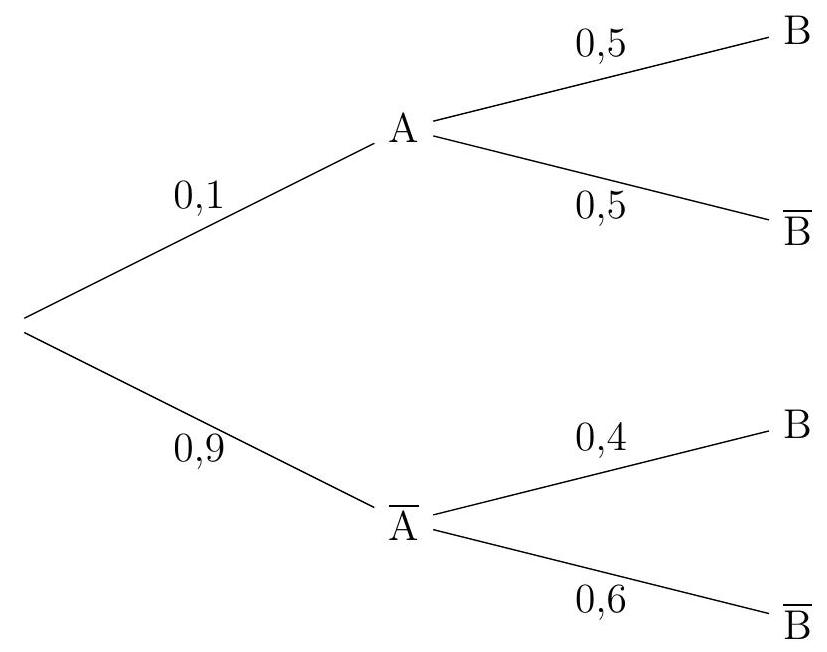
\includegraphics[max width=0.35\textwidth, center]{2025_05_13_795d2fb7a2e4fd469256g-6}
% \vspace{-2em}
% 
% Déterminer $\mathrm{P}(\mathrm{B})$.
% ~\\Solution :
% D'après la formule des probabilités totales :
% $$
% \begin{aligned}
% \mathrm{P}(\mathrm{B}) & =\mathrm{P}(\mathrm{A} \cap \mathrm{B})+\mathrm{P}(\overline{\mathrm{A}} \cap \mathrm{B}) \\
% & =\mathrm{P}(\mathrm{A}) \times \mathrm{P}_{\mathrm{A}}(\mathrm{~B})+\mathrm{P}(\overline{\mathrm{A}}) \times \mathrm{P}_{\overline{\mathrm{A}}}(\mathrm{B}) \\
% & =0,1 \times 0,5+0,9 \times 0,4 \\
% & =0,41
% \end{aligned}
% $$
% \end{example}
% 
% \begin{method}{Déterminer des probabilités}{}
% \begin{itemize}
%   \item Faire un tableau (plutôt lorsqu'on connait les probabilités des intersections)
%   \item Faire un arbre (plutôt lorsqu'on connait les probabilités conditionnelles)
% \end{itemize}
% \end{method}
% 
% % \subsection{Calculer $\mathrm{P}_{\mathrm{B}}(\mathrm{A})$ lorsqu'on connait $\mathrm{P}_{\mathrm{A}}(\mathrm{B})$}
% % \begin{method}{Calculer $\mathrm{P}_{\mathrm{B}}(\mathrm{A})$ lorsqu'on connait $\mathrm{P}_{\mathrm{A}}(\mathrm{B})$}{}
% % \begin{itemize}
% %   \item Écrire la définition de $\mathrm{P}_{\mathrm{B}}(\mathrm{A})$ :
% % \end{itemize}
% % 
% % $$
% % P_{\mathrm{B}}(\mathrm{A})=\frac{P(\mathrm{A} \cap \mathrm{B})}{P(\mathrm{B})} .
% % $$
% % 
% % \begin{itemize}
% %   \item Calculer $\mathrm{P}(\mathrm{A} \cap \mathrm{B})$ grâce à $\mathrm{P}_{\mathrm{A}}(\mathrm{B})$.
% %   \item Calculer $\mathrm{P}(\mathrm{B})$ avec la formule des probabilités totales.
% % \end{itemize}
% % \end{method}
% % 
% % \begin{example}
% % Un sondage effectué dans une région montagneuse à propos de la construction d'un barrage donne les résultats suivants :
% % 
% % \begin{itemize}
% %   \item 65\% des personnes intérrogées sont contre la construction du barrage;
% %   \item Parmi les personnes qui sont contre cette construction, $70 \%$ sont des écologistes.
% %   \item Parmi les personnes qui sont favorables à la construction, $20 \%$ sont des écologistes. Quelle est la proportion de personnes contre le barrage parmi les écologistes?
% % \end{itemize}
% % 
% % ~\\Solution :
% % 
% % On note $C$ l'événement «La personne interrogée est contre la construction» et $E$ l'événement «La personne interrogée est écologiste».\\
% % On souhaite déterminer $\mathrm{P}_{E}(C)=\dfrac{\mathrm{P}(E \cap C)}{\mathrm{P}(E)}$.\\
% % On représente la situation par l'arbre suivant :\\
% % 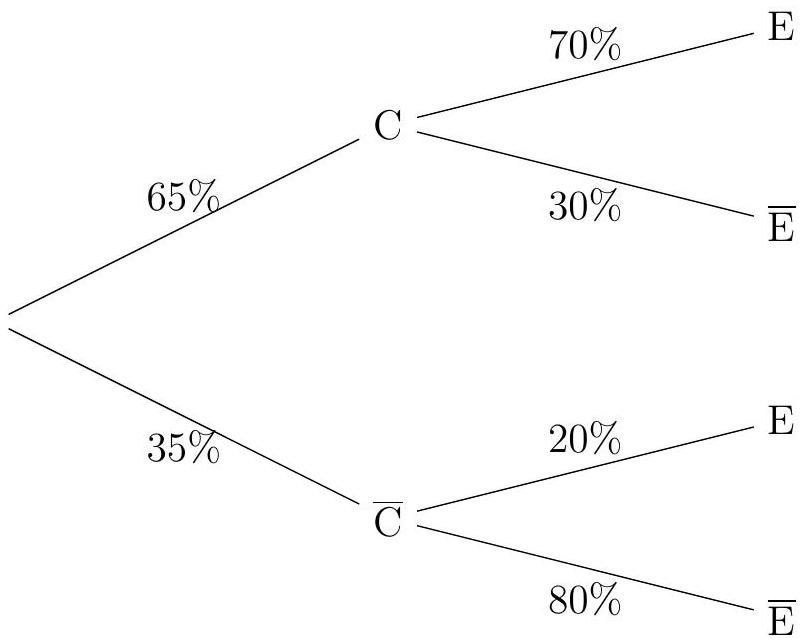
\includegraphics[max width=0.4\textwidth, center]{2025_05_13_795d2fb7a2e4fd469256g-7}
% % 
% % D'une part, on voit sur l'arbre que $\mathrm{P}(\mathrm{E} \cap \mathrm{C})=65 \% \times 70 \%=45,5 \%$.\\
% % D'autre part, d'après la formule des probabilités totales :
% % 
% % $$
% % \begin{aligned}
% % \mathrm{P}(\mathrm{E}) & =\mathrm{P}(\mathrm{E} \cap \mathrm{C})+\mathrm{P}(\mathrm{E} \cap \overline{\mathrm{C}}) \\
% % & =65 \% \times 70 \%+35 \% \times 20 \% =52,5 \%
% % \end{aligned}
% % $$
% % 
% % Finalement, on a :
% % 
% % $$
% % P_{E}(C)=\frac{P(E \cap C)}{P(E)}=\frac{45,5 \%}{52,5 \%} \simeq 86,7 \% .
% % $$
% % 
% % Il y a donc environ 86,7\% de personnes contre le barrage parmi les écologistes.
% % \end{example}
% 
% \section{Indépendance d'événements}
% \begin{definition}{Indépendance}{}
% Soient A et B deux événements. On dit que A et B sont \textbf{indépendants} lorsque :
% 
% $$
% \mathrm{P}(\mathrm{A} \cap \mathrm{B})=\hideM{\mathrm{P}(\mathrm{A}) \times \mathrm{P}(\mathrm{B})}
% $$
% 
% \end{definition}
% \begin{example}
% Soient A et B deux événements tels que $\mathrm{P}(\mathrm{A})=0,3, \mathrm{P}(\mathrm{B})=0,2$ et $\mathrm{P}(\mathrm{A} \cap \mathrm{B})=0,7$. Les événements $A$ et $B$ sont-ils indépendants?
% ~\\Solution :
% 
% $\mathrm{P}(\mathrm{A}) \times \mathrm{P}(\mathrm{B})=0,2 \times 0,3=0,06 \neq \mathrm{P}(\mathrm{A} \cap \mathrm{B})$.\\
% On en déduit que les événements A et B ne sont pas indépendants.
% \end{example}
% 
% \begin{proposition}{}{}
% Soient A et B deux événements avec $\mathrm{P}(\mathrm{A}) \neq 0$.\\
% A et B sont indépendants si, et seulement si,
% 
% $$
% \mathrm{P}_{\mathrm{A}}(\mathrm{B})=\hideM{\mathrm{P}(\mathrm{B})}
% $$
% \end{proposition}
% 
% \begin{demo}
% $\mathrm{P}(\mathrm{A}) \neq 0$ donc $\mathrm{P}_{\mathrm{A}}(\mathrm{B})=\dfrac{\mathrm{P}(\mathrm{A} \cap \mathrm{B})}{\mathrm{P}(\mathrm{A})}$, c'est-à-dire $\mathrm{P}(\mathrm{A} \cap \mathrm{B})=\mathrm{P}(\mathrm{A}) \times \mathrm{P}_{\mathrm{A}}(\mathrm{B})$.\\
% Ainsi, on a les équivalences suivantes :
% 
% $$
% \begin{aligned}
% \text { A et } \mathrm{B} \text { sont indépendants } & \Longleftrightarrow \mathrm{P}(\mathrm{A} \cap \mathrm{B})=\mathrm{P}(\mathrm{A}) \times \mathrm{P}(\mathrm{B}) \\
% & \Longleftrightarrow \mathrm{P}(\mathrm{A}) \times \mathrm{P}_{\mathrm{A}}(\mathrm{B})=\mathrm{P}(\mathrm{A}) \times \mathrm{P}(\mathrm{B}) \\
% & \Longleftrightarrow \mathrm{P}_{\mathrm{A}}(\mathrm{B})=\mathrm{P}(\mathrm{B}) \quad(\operatorname{car} \mathrm{P}(\mathrm{A}) \neq 0)
% \end{aligned}
% $$
% \end{demo}
% 
% \begin{proposition}{}{}
% Si $\mathrm{A}$ et $\mathrm{B}$ sont indépendants, alors les événements $\mathrm{A}$ et $\overline{\mathrm{B}}$ sont également indépendants.
% \end{proposition}
% 
% \begin{demo}
% D'après la formule des probabilités totales :
% 
% $$
% \mathrm{P}(\mathrm{A})=\mathrm{P}(\mathrm{A} \cap \mathrm{B})+\mathrm{P}(\mathrm{A} \cap \overline{\mathrm{B}})
% $$
% 
% Par indépendance de A et B, on a :
% \vspace{-2em}
% 
% \begin{align*}
% \mathrm{P}(\mathrm{~A})=\mathrm{P}(\mathrm{A}) \times \mathrm{P}(\mathrm{B})+\mathrm{P}(\mathrm{A} \cap \overline{\mathrm{B}}) &\Longleftrightarrow \mathrm{P}(\mathrm{A})(1-\mathrm{P}(\mathrm{B}))=\mathrm{P}(\mathrm{A} \cap \overline{\mathrm{B}}) \\
% &\Longleftrightarrow \mathrm{P}(\mathrm{A}) \mathrm{P}(\overline{\mathrm{B}})=\mathrm{P}(\mathrm{A} \cap \overline{\mathrm{B}})
% \end{align*}
% 
% Cela signifie exactement que A et $\overline{\mathrm{B}}$ sont également indépendants.
% \end{demo}

\begin{savoir}{}{}
\begin{itemize}
  \item Passer du registre de la langue naturelle au registre symbolique et inversement.
  \item Calculer une probabilité conditionnelle.
  %\item Utiliser la formule des probabilités totales (en particulier avec un arbre).
  \item Construire et utiliser un arbre ou un tableau pour résoudre un problème.
  %\item Distinguer $\mathrm{P}_{\mathrm{A}}(\mathrm{B})$ et $\mathrm{P}_{\mathrm{B}}(\mathrm{A})$ dans des problèmes de type «faux-positifs».
  %\item Déterminer et utiliser l'indépendance de deux événements.
\end{itemize}
\end{savoir}


\end{document}